%%
% Copyright (c) 2017, Pascal Wagler;  
% Copyright (c) 2014--2017, John MacFarlane
% 
% All rights reserved.
% 
% Redistribution and use in source and binary forms, with or without 
% modification, are permitted provided that the following conditions 
% are met:
% 
% - Redistributions of source code must retain the above copyright 
% notice, this list of conditions and the following disclaimer.
% 
% - Redistributions in binary form must reproduce the above copyright 
% notice, this list of conditions and the following disclaimer in the 
% documentation and/or other materials provided with the distribution.
% 
% - Neither the name of John MacFarlane nor the names of other 
% contributors may be used to endorse or promote products derived 
% from this software without specific prior written permission.
% 
% THIS SOFTWARE IS PROVIDED BY THE COPYRIGHT HOLDERS AND CONTRIBUTORS 
% "AS IS" AND ANY EXPRESS OR IMPLIED WARRANTIES, INCLUDING, BUT NOT 
% LIMITED TO, THE IMPLIED WARRANTIES OF MERCHANTABILITY AND FITNESS 
% FOR A PARTICULAR PURPOSE ARE DISCLAIMED. IN NO EVENT SHALL THE 
% COPYRIGHT OWNER OR CONTRIBUTORS BE LIABLE FOR ANY DIRECT, INDIRECT, 
% INCIDENTAL, SPECIAL, EXEMPLARY, OR CONSEQUENTIAL DAMAGES (INCLUDING,
% BUT NOT LIMITED TO, PROCUREMENT OF SUBSTITUTE GOODS OR SERVICES; 
% LOSS OF USE, DATA, OR PROFITS; OR BUSINESS INTERRUPTION) HOWEVER 
% CAUSED AND ON ANY THEORY OF LIABILITY, WHETHER IN CONTRACT, STRICT 
% LIABILITY, OR TORT (INCLUDING NEGLIGENCE OR OTHERWISE) ARISING IN 
% ANY WAY OUT OF THE USE OF THIS SOFTWARE, EVEN IF ADVISED OF THE 
% POSSIBILITY OF SUCH DAMAGE.
%%

%%
% For usage information and examples visit the GitHub page of this template:
% https://github.com/Wandmalfarbe/pandoc-latex-template
%%

\PassOptionsToPackage{unicode=true}{hyperref} % options for packages loaded elsewhere
\PassOptionsToPackage{hyphens}{url}
%
\documentclass[american,a4paper,oneside,,tablecaptionabove]{scrbook}
\usepackage{lmodern}
\usepackage{amssymb,amsmath}
\usepackage{ifxetex,ifluatex}
\usepackage{fixltx2e} % provides \textsubscript
\ifnum 0\ifxetex 1\fi\ifluatex 1\fi=0 % if pdftex
  \usepackage[T1]{fontenc}
  \usepackage[utf8]{inputenc}
  \usepackage{textcomp} % provides euro and other symbols
\else % if luatex or xelatex
  \usepackage{unicode-math}
  \defaultfontfeatures{Ligatures=TeX,Scale=MatchLowercase}
\fi
% use upquote if available, for straight quotes in verbatim environments
\IfFileExists{upquote.sty}{\usepackage{upquote}}{}
% use microtype if available
\IfFileExists{microtype.sty}{%
\usepackage[]{microtype}
\UseMicrotypeSet[protrusion]{basicmath} % disable protrusion for tt fonts
}{}
\IfFileExists{parskip.sty}{%
\usepackage{parskip}
}{% else
\setlength{\parindent}{0pt}
\setlength{\parskip}{6pt plus 2pt minus 1pt}
}
\usepackage{hyperref}
\hypersetup{
            pdftitle={Development of an interactive dashboard for performance reports on IBM Z systems with Linux},
            pdfauthor={Paul Bauriegel},
            pdfborder={0 0 0},
            breaklinks=true}
\urlstyle{same}  % don't use monospace font for urls
\usepackage[margin=2.5cm,includehead=true,includefoot=true,centering]{geometry}
\usepackage{listings}
\newcommand{\passthrough}[1]{#1}
\usepackage{graphicx,grffile}
\makeatletter
\def\maxwidth{\ifdim\Gin@nat@width>\linewidth\linewidth\else\Gin@nat@width\fi}
\def\maxheight{\ifdim\Gin@nat@height>\textheight\textheight\else\Gin@nat@height\fi}
\makeatother
% Scale images if necessary, so that they will not overflow the page
% margins by default, and it is still possible to overwrite the defaults
% using explicit options in \includegraphics[width, height, ...]{}
\setkeys{Gin}{width=\maxwidth,height=\maxheight,keepaspectratio}
\setlength{\emergencystretch}{3em}  % prevent overfull lines
\providecommand{\tightlist}{%
  \setlength{\itemsep}{0pt}\setlength{\parskip}{0pt}}
\setcounter{secnumdepth}{0}
% Redefines (sub)paragraphs to behave more like sections
\ifx\paragraph\undefined\else
\let\oldparagraph\paragraph
\renewcommand{\paragraph}[1]{\oldparagraph{#1}\mbox{}}
\fi
\ifx\subparagraph\undefined\else
\let\oldsubparagraph\subparagraph
\renewcommand{\subparagraph}[1]{\oldsubparagraph{#1}\mbox{}}
\fi

% Make use of float-package and set default placement for figures to H
\usepackage{float}
\floatplacement{figure}{H}

\ifnum 0\ifxetex 1\fi\ifluatex 1\fi=0 % if pdftex
  \usepackage[shorthands=off,main=american]{babel}
\else
    % See issue https://github.com/reutenauer/polyglossia/issues/127
  \renewcommand*\familydefault{\sfdefault}
    % load polyglossia as late as possible as it *could* call bidi if RTL lang (e.g. Hebrew or Arabic)
  \usepackage{polyglossia}
  \setmainlanguage[variant=american]{english}
\fi

\title{Development of an interactive dashboard for performance reports on IBM Z
systems with Linux}
\providecommand{\subtitle}[1]{}
\subtitle{Term Paper T3000}
\author{Paul Bauriegel}
\date{}





%%
%% added
%%

%
% No language specified? take American English.
%


%
% colors
%
\usepackage[dvipsnames,svgnames*,x11names*,table]{xcolor}

%
% listing colors
%
\definecolor{listing-background}{HTML}{F7F7F7}
\definecolor{listing-rule}{HTML}{B3B2B3}
\definecolor{listing-numbers}{HTML}{B3B2B3}
\definecolor{listing-text-color}{HTML}{000000}
\definecolor{listing-keyword}{HTML}{435489}
\definecolor{listing-identifier}{HTML}{435489}
\definecolor{listing-string}{HTML}{00999A}
\definecolor{listing-comment}{HTML}{8E8E8E}
\definecolor{listing-javadoc-comment}{HTML}{006CA9}

%\definecolor{listing-background}{rgb}{0.97,0.97,0.97}
%\definecolor{listing-rule}{HTML}{B3B2B3}
%\definecolor{listing-numbers}{HTML}{B3B2B3}
%\definecolor{listing-text-color}{HTML}{000000}
%\definecolor{listing-keyword}{HTML}{D8006B}
%\definecolor{listing-identifier}{HTML}{000000}
%\definecolor{listing-string}{HTML}{006CA9}
%\definecolor{listing-comment}{rgb}{0.25,0.5,0.35}
%\definecolor{listing-javadoc-comment}{HTML}{006CA9}

%
% for the background color of the title page
%
\usepackage{pagecolor}
\usepackage{afterpage}

%
% TOC depth and 
% section numbering depth
%
\setcounter{tocdepth}{3}

%
% line spacing
%
\usepackage{setspace}
\setstretch{1.2}

%
% break urls
%
\PassOptionsToPackage{hyphens}{url}

%
% When using babel or polyglossia with biblatex, loading csquotes is recommended 
% to ensure that quoted texts are typeset according to the rules of your main language.
%
\usepackage{csquotes}

%
% captions
%
\definecolor{caption-color}{HTML}{777777}
\usepackage[font={stretch=1.2}, textfont={color=caption-color}, position=top, skip=4mm, labelfont=bf, singlelinecheck=false, justification=raggedright]{caption}
\setcapindent{0em}
\captionsetup[longtable]{position=above}

%
% blockquote
%
\definecolor{blockquote-border}{RGB}{221,221,221}
\definecolor{blockquote-text}{RGB}{119,119,119}
\usepackage{mdframed}
\newmdenv[rightline=false,bottomline=false,topline=false,linewidth=3pt,linecolor=blockquote-border,skipabove=\parskip]{customblockquote}
\renewenvironment{quote}{\begin{customblockquote}\list{}{\rightmargin=0em\leftmargin=0em}%
\item\relax\color{blockquote-text}\ignorespaces}{\unskip\unskip\endlist\end{customblockquote}}

%
% Source Sans Pro as the de­fault font fam­ily
% Source Code Pro for monospace text
%
% 'default' option sets the default 
% font family to Source Sans Pro, not \sfdefault.
%
\usepackage[default]{sourcesanspro}
\usepackage{sourcecodepro}

%
% heading color
%
\definecolor{heading-color}{RGB}{40,40,40}
\addtokomafont{section}{\color{heading-color}}
% When using the classes report, scrreprt, book, 
% scrbook or memoir, uncomment the following line.
%\addtokomafont{chapter}{\color{heading-color}}

%
% variables for title and author
%
\usepackage{titling}
\title{Development of an interactive dashboard for performance reports on IBM Z
systems with Linux}
\author{Paul Bauriegel}

%
% tables
%

%
% remove paragraph indention
%
\setlength{\parindent}{0pt}
\setlength{\parskip}{6pt plus 2pt minus 1pt}
\setlength{\emergencystretch}{3em}  % prevent overfull lines

%
%
% Listings
%
%

\lstdefinestyle{eisvogel_listing_style}{
  language         = java,
  numbers          = left,
  backgroundcolor  = \color{listing-background},
  basicstyle       = \color{listing-text-color}\small\ttfamily{}\linespread{1.15}, % print whole listing small
  xleftmargin      = 2.7em,
  breaklines       = true,
  frame            = single,
  framesep         = 0.6mm,
  rulecolor        = \color{listing-rule},
  frameround       = ffff,
  framexleftmargin = 2.5em,
  tabsize          = 4,
  numberstyle      = \color{listing-numbers},
  aboveskip        = 1.0em,
  keywordstyle     = \color{listing-keyword}\bfseries,
  classoffset      = 0,
  sensitive        = true,
  identifierstyle  = \color{listing-identifier},
  commentstyle     = \color{listing-comment},
  morecomment      = [s][\color{listing-javadoc-comment}]{/**}{*/},
  stringstyle      = \color{listing-string},
  showstringspaces = false,
  escapeinside     = {/*@}{@*/}, % Allow LaTeX inside these special comments
  literate         =
  {á}{{\'a}}1 {é}{{\'e}}1 {í}{{\'i}}1 {ó}{{\'o}}1 {ú}{{\'u}}1
  {Á}{{\'A}}1 {É}{{\'E}}1 {Í}{{\'I}}1 {Ó}{{\'O}}1 {Ú}{{\'U}}1
  {à}{{\`a}}1 {è}{{\'e}}1 {ì}{{\`i}}1 {ò}{{\`o}}1 {ù}{{\`u}}1
  {À}{{\`A}}1 {È}{{\'E}}1 {Ì}{{\`I}}1 {Ò}{{\`O}}1 {Ù}{{\`U}}1
  {ä}{{\"a}}1 {ë}{{\"e}}1 {ï}{{\"i}}1 {ö}{{\"o}}1 {ü}{{\"u}}1
  {Ä}{{\"A}}1 {Ë}{{\"E}}1 {Ï}{{\"I}}1 {Ö}{{\"O}}1 {Ü}{{\"U}}1
  {â}{{\^a}}1 {ê}{{\^e}}1 {î}{{\^i}}1 {ô}{{\^o}}1 {û}{{\^u}}1
  {Â}{{\^A}}1 {Ê}{{\^E}}1 {Î}{{\^I}}1 {Ô}{{\^O}}1 {Û}{{\^U}}1
  {œ}{{\oe}}1 {Œ}{{\OE}}1 {æ}{{\ae}}1 {Æ}{{\AE}}1 {ß}{{\ss}}1
  {ç}{{\c c}}1 {Ç}{{\c C}}1 {ø}{{\o}}1 {å}{{\r a}}1 {Å}{{\r A}}1
  {€}{{\EUR}}1 {£}{{\pounds}}1 {«}{{\guillemotleft}}1
  {»}{{\guillemotright}}1 {ñ}{{\~n}}1 {Ñ}{{\~N}}1 {¿}{{?`}}1
  {…}{{\ldots}}1 {≥}{{>=}}1 {≤}{{<=}}1 {„}{{\glqq}}1 {“}{{\grqq}}1
  {”}{{''}}1
}
\lstset{style=eisvogel_listing_style}

\lstdefinelanguage{XML}{
  morestring      = [b]",
  moredelim       = [s][\bfseries\color{listing-keyword}]{<}{\ },
  moredelim       = [s][\bfseries\color{listing-keyword}]{</}{>},
  moredelim       = [l][\bfseries\color{listing-keyword}]{/>},
  moredelim       = [l][\bfseries\color{listing-keyword}]{>},
  morecomment     = [s]{<?}{?>},
  morecomment     = [s]{<!--}{-->},
  commentstyle    = \color{listing-comment},
  stringstyle     = \color{listing-string},
  identifierstyle = \color{listing-identifier}
}

%
% header and footer
%
\usepackage{fancyhdr}
\pagestyle{fancy}
\fancyhead{}
\fancyfoot{}
\lhead{Development of an interactive dashboard for performance reports on IBM Z
systems with Linux}
\chead{}
\rhead{}
\lfoot{Paul Bauriegel}
\cfoot{}
\rfoot{\thepage}
\renewcommand{\headrulewidth}{0.4pt}
\renewcommand{\footrulewidth}{0.4pt}

%%
%% end added
%%

\begin{document}

%%
%% begin titlepage
%%

\begin{titlepage}
\newgeometry{left=6cm}
\definecolor{titlepage-color}{HTML}{25467a}
\newpagecolor{titlepage-color}\afterpage{\restorepagecolor}
\newcommand{\colorRule}[3][black]{\textcolor[HTML]{#1}{\rule{#2}{#3}}}
\begin{flushleft}
\noindent
\\[-1em]
\color[HTML]{ffffff}
\makebox[0pt][l]{\colorRule[ffffff]{1.3\textwidth}{1pt}}
\par
\noindent

{ \setstretch{1.4}
\vfill
\noindent {\huge \textbf{\textsf{Development of an interactive dashboard for performance reports on IBM Z
systems with Linux}}}
\vskip 1em
{\Large \textsf{Term Paper T3000}}
\vskip 2em
\noindent
{\Large \textsf{\MakeUppercase{Paul Bauriegel}}
\vfill
}

\textsf{}}
\end{flushleft}
\end{titlepage}
\restoregeometry

%%
%% end titlepage
%%


{
\setcounter{tocdepth}{2}
\tableofcontents
}
\chapter{Introduction}\label{introduction}

Data is a valuable resource (1), especially when analyzing or comparing
the performance of different technologies. With test data, it's possible
to find bottlenecks in applications or errors in the process flow.
However, most large data set are useless until there have been evaluated
or visualized to gain insights. The visualization makes it easier for
the analyst to understand the relations and evolutions inside the data.
As result, it makes his work more efficient. Nevertheless, visualization
takes valuable time, especially when it has to be done over and over
again. There are several software solutions on the market
{[}Meek.2017{]} to automate these visualizations and get fast insights,
like \emph{Tableau} or \emph{Voyager 2} ({\textbf{???}}). But there are
also circumstances which require highly customized reports, as it is
necessary for the \emph{IBM z Linux Performance} department.\\
The \emph{IBM z Linux Performance} department has several test
procedures to evaluate the IBM Z Mainframes on Linux for several
workloads. These test runs result in different kinds of reports. By now
these reports had to be manually analyzed. The goal of this project is
to support the performance analysists by creating an interactive
dashboard for their requirements. The dashboard aims to automate the
process of visualization without losing the flexibility in the data
presentation.

This paper presents a working dashboard with specialized performance
visualizations. It discusses the design choices for technology and
architecture in this application and the ideas behind the different
visualizations. The report highlights the advantages of this tool as
well as further challenges.

Therefore the reader will be introduced to the design aspects of data
visualization and the requirements for an interactive performance
visualization dashboard. The first chapter explains how effective data
visualization has to be implemented. The second provides a case study
for the application, which includes detailed information about the data
source.\\
On this foundation, the technologies and architecture of the application
will be explained. The part compares the different technology options
and underlines the design decisions.\\
Based on the architecture the dashboard prototype will be explained and
which further improvements could be implemented.

\chapter{Concepts of data
visualization}\label{concepts-of-data-visualization}

\section{What means data
visualization}\label{what-means-data-visualization}

Visualization meant in its original sense to \enquote{construct a visual
image in the mind} ({\textbf{???}}). In the computer science the
understanding for this term is different, as Earnshaw defines it:\\
\enquote{Scientific Visualization is concerned with exploring data and
information in such a way as to gain understanding and insight into the
data.} ({\textbf{???}})\\
The term is now referring to building an visual image based on data. In
a more general context its data visualization. There are multiple
definitions for the term data visualization on different levels of
abstraction ({\textbf{???}}). In the words of Ignatius and Senay:\\
\enquote{The primary objective in data visualization is to gain insight
into an information space.} ({\textbf{???}})\\
Data visualization has varieties like in information or scientific
visualization {[}Friendly{]}. These terms have a slightly different
semantical definition. Information visualization is more precise,
because it presents the data in a specific interpretation context (S.
4f, {\textbf{???}}). The term scientific visualization is mostly used in
the context of visualization for science research ({\textbf{???}}).
Because the distinction is not relevant for this paper, the terms will
be used equally in the further chapters.\\
The dashboard described in this paper is a tool for information
visualization. Therefore information visualization will be described
shortly. According to Gershon information visualization
\enquote{combines aspects of scientific visualization, human-computer
interfaces, data mining, imaging and graphics} ({\textbf{???}}).\\
Information visualization has two main goal ({\textbf{???}}):

\begin{itemize}
\item
  data representation, by transferring the data in a suitable layout for
  presentation
\item
  data exploration or visual data mining, discovery of new knowledge by
  transforming and interconnecting the data.
\end{itemize}

The data representation should allow to find and view the data on
specific criteria. The representation should contain multiple views on
the selection with a different context. The representation easy to keep
in mind, to support the analyst.\\
The data exploration should highlight relations and structures in the
data. To find insights multiple data sets should be interconnect-able.
({\textbf{???}})

\section{The process of data
visualization}\label{the-process-of-data-visualization}

Russell Ackoff defines the process of discovering new knowledge in three
abstract levels for the perceptual and cognitive space ({\textbf{???}}).
The paper by Chen et al. extends these definitions for the computational
space ({\textbf{???}}). These levels are:\\
Data - Data is a concatenation of different symbols, for example
strings. In the computer science data can by any stored representations
of a models or an attributes in the memory.\\
Information - Information is processed data that has been given a
context. The context can be assigned by either a computational process
or humans annotating the data.\\
Knowledge - Knowledge is an application of data and information to
understand the processes and developments that created the data. This
can be the results of av machine learning process or analysis by subject
matter experts.\\
Understanding - Understanding extends the knowledge by providing
explanations for the developments in the data.

\begin{figure}
\centering
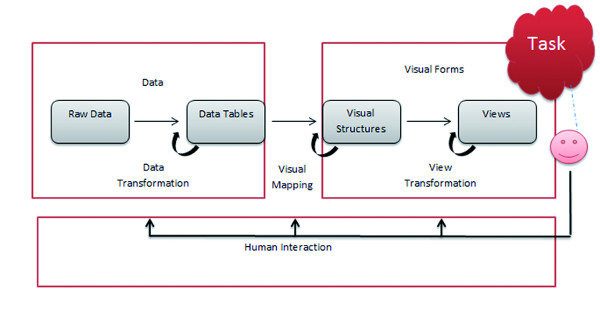
\includegraphics{images/krypczyk_diagrammarten_1.jpg}
\caption{Process of visualization}
\end{figure}

The process of visualization has been defined in a reference model by
Card, Mackinlay and Shneiderman ({\textbf{???}}, \textbf{???},
\textbf{???}). The model has three transformation phases, to transform
the data between the different levels of knowledge. In in the beginning
the raw data is transformed in structured tables. Data in tabular form
is easier to visualize. The \emph{data} becomes \emph{information}.\\
The visual mapping converts the data tables into visual structures.
These have graphical properties instead of the mathematical relation
inside the tables. The mapping into structures results in possible
\emph{knowledge} for the viewer. Such a mapping depends on the chosen
chart type and if the data is discrete or continuous.\\
In the last transformation step, the visualization is adjusted to
highlight parts of the data and get a better \emph{understanding}. On a
user driven dashboard, the user \textbf{interacts with the
visualization} to create different views.

The model has also been refined by dos Santos ({\textbf{???}}), adding
new data filtering step after the general data transformations. In the
option of the author this model over specified for most modern use
cases, where big data sets are evaluated in real time and can be
filtered in the frontend. Furthermore the model is specialized on
generating images. When the visualization is rendered for example on the
server side this model is applicable, but in a modern visualization
frontend, the visualization doesn't have to be a picture or in Ben
Shneidermans words: \enquote{The purpose of visualization is insight,
not pictures.} ({\textbf{???}})

\section{Visualization best
practices}\label{visualization-best-practices}

In an interactive dashboard the user can adjust his view of the data,
but not the kind of representation. The representation type is stills
defined in the visual structures. Best practices for visualization help
to develop an appealing visual mapping for the data. The chapter
summarizes the Graphical excellence points laid out by Edward Tufte
({\textbf{???}}, S.13, \textbf{???}).

\emph{Show the complete data} - Provide the data source, with its
limitations\\
\emph{Data over Visualization} - Encourage the viewer to think about the
substance rather than it's representation or methodology\\
\emph{Assume an Intelligent Audience} - Don't oversimplify the data or
the visualization, induce the viewer to think about the data\\
\emph{Encourage data exploration} - show the data at several levels of
detail, from broad overview to the fine structure, enable comparisons
for different pieces of data\\
\\
\emph{Make data understandable} - integrate verbal descriptions in the
dataset, avoid distorting what the data have to say and follow
conventions when presenting the data.\\
\emph{Avoid confusing charts} - choosing the wrong representation can
unintentionally confuse or deliberately mislead the viewer.

\section{Choosing the best chart
type}\label{choosing-the-best-chart-type}

How easily the user is able to work with the data depends mainly on the
type of chart. Mackinlay and Tufte use their publication to explain
their selection of visualization type based on sets of examples. This
paper will not summarize their main works. Instead it will use simple
classifications guidelines for the choice of visualization. To decide if
either a chart or another representation is used, the Visual Thinking
Codex by Dan Roam will be applied. This paper expects that all data will
represented as chart. Because of that a chart selection diagram by
Andrew Abela should help to use the best chart visualization
({\textbf{???}}).

The Visual Thinking Codex is a tool for visual thinking by Dan Roam
({\textbf{???}}). Visual thinking is methodology to organize the
thoughts by visualizing them. The codex is using another tool called
SQVID. The idea behind SQVID is that your can think of thing in a
variety of different ways. \textbf{S}imple or Elaborate,
\textbf{Q}ualitative vs Quantitative, \textbf{V}ision and Execution,
\textbf{I}ndividual against Comparison, \textbf{D}ifference/change or As
is. ({\textbf{???}})\\
The codex suggest different types of visualization. The decision is
based on the question that should answer and kind focus in the SQVID
methodology.\\
Any z performance analyst ask primarily two kinds of question \emph{How}
is sth. or \emph{Why} is it like this. For example \emph{How} much
memory is used?, or \emph{Why} are we loosing performance?. These
question come form different view angles, so that no filtering based on
the kind thinking can by made. But on the questions only it can be seen
that plots and charts are the primary visualization type. Therefore a
further chart study can provide some advice for choosing the right
chart. ({\textbf{???}})

As part of the Extreme Presentation \textsuperscript{TM} Method Abela
did provide a Chart Suggestion graphic which can help to chose the right
presentation method. The main question is after what should be shown. An
comparison can be shown with bar or column charts. Distribution may be
better with histograms. A relationship requires a bubble or scatter
chart and a composition can be shown with stacked or pie charts. This
source is just meant to be a simple overview and is not in any meaning
complete. ({\textbf{???}})

Good resources ({\textbf{???}}) for a more detailed exploration of
graphs are the following. For the fundamentals of graph design
\enquote{Show Me the Numbers} by Stephen few is a helpful resource. The
best encyclopedic reference for visualization is \enquote{Information
Graphics} by Robert Harris. For a even more detailed exploration of
visualization \enquote{The Visual Display of Quantitative Information}
by Edward ({\textbf{???}}) and \enquote{The Elements of Graphing Data}
by William Cleveland can be used.\\
The \enquote{perception edge} blog ({\textbf{???}}) provides a
collection of different papers, with solutions for more or less common
problems when developing chart. Some of these suggestion will be used in
the further implementation.

\chapter{Use case study of the application
requirements}\label{use-case-study-of-the-application-requirements}

Building a good visualization is not easy. To build the perfect
visualization this chapter will introduce design principles, processed
and an overview how the actual data looks like. Together these
information should help to develop an dashboard on the needs of the user
and with the right processes or technologies.

\section{Use Case Analytics with User Experience
principles}\label{use-case-analytics-with-user-experience-principles}

Choosing a matching visualization type makes the data understandable.
According to Tufte good graphics are furthermore encouraging the viewers
also to explore the data set. Therefore this paper is proposing an
interactive dashboard. To ensure the best user experience on the
dashboard, this chapter will introduce the User Interface (UI) Design
and User Experience (UX) Design. In simple words is UI how things
\textbf{look} and UX how things \textbf{work}. ({\textbf{???}}) This
chapter will outline the main UI design principles and which UX
processes help to develop the best user experience.

\subsection{UI design principles}\label{ui-design-principles}

Good UI design and suitable design principles have been defined by many
authors over the time. The paper will cite three publications on
different degree of details. At first the main principles of design will
be presented based on the Donald Normans book \enquote{The Design of
Everyday Things}. Than these principles will be specialized for the UI
design. At last the principles of website design will be explained based
on \enquote{Don't Make Me Think} by Steve Krug.

Thinking about the design of a product before building it, results in
more user-friendly products. Norman provides seven principles, which
good designers should follow.\\

\emph{Provide the Necessary Knowledge} - The user build his own
conceptual model how the thing is working. Good design provides the
information to interpret and understand the object. It contains visible
clues for their function.\\
\emph{Simplify} - The complexity of the product increases as the square
of the features. To simplify tasks four methods, can be used. Provide
the user a simple, intuitive mental aid. Show feedback to the user
instead of making they remembering things. Third and Fourth, automate
functions and change the way of presenting the information.\\
\emph{Show How to Use a Tool and Explain Its State} - The user should
know about the consequences of their actions and the devices gave them
feedback promptly.\\
\emph{Map Correctly} - Developing a product should consider the user's
natural mappings (e.g. \enquote{up} more naturally suggests
\enquote{louder} than does \enquote{left})\\
\emph{Use Constraints} - Contains help to understand the product. The
lead the user to use the product in the correct way.\\
\emph{Expect Errors} - If the user can create an error, it's very likely
he will do so. Good design prevents as much errors as possible and gives
informative feedback, for those than cannot be prevented. Most errors
are either \enquote{slips} or \enquote{mistakes.} Slips are errors by
accident, like throwing the wrong document in the trash. Mistakes, on
the other hand, are conscious actions, taken by having the wrong goal or
misleading information.\\
\emph{Consider Standardizing} - Standard are useful because they base
your application on a ground of common knowledge for all user. Consider
a car, wherever on the word you take a car, there are all operating same
way.

For User Interfaces the core practices concentrate more on the style
aspects of the application. There a five key principles a good UI is
measured on ({\textbf{???}}).\\
\emph{Color} - The color is influencing the emotions of the viewer. Some
meanings of colors are predefined like red for attention. Knowing about
the psychology of colors is important. Principles of color do also
include using matching color schemes for charts or web elements.
({\textbf{???}})\\
\emph{Balance} - Balance in the design context is arranging elements to
establish a positive communication to the user. Getting interest and
positive feedback by the user is achieved by multiple criteria, like
symmetry, asymmetry, or alignment. ({\textbf{???}})\\
\emph{Contrast} - Contrast is used for three main reasons. 1. Contrast
is attractive to the eye, 2. It helps to organize information or build a
hierarchy, 3. The Contrast moves elements in the focus of the viewer.
({\textbf{???}})\\
\emph{Typography} - Fonts and the content itself are the main influence
how users process the given information. Therefore the should by chosen
with caution. ({\textbf{???}})\\
\emph{Consistency} - Consistency is the key principle in UI design. It
makes the product intuitive, usable and eliminates confusion.
Consistency is based on familiar patterns and common visuals like color
schemes, same typography or spaces between elements. ({\textbf{???}})

This work will create a User Interface in the web as explained further
in chapter \textbf{XY}. Steven Krug did summarize the key principles for
website Design in his book. To get a basic understanding about good
Website Design his core point will here be summarized.

\emph{Create a clear visual hierarchy} -- Like defined by consistency
principle the web page should \enquote{clearly and accurately portray
the relationships among the things on the page.}. If elements are
conceptually linked, they are visually linked as well. Important aspects
are highlighted with visual cues, like bold or larger fonts.\\
\emph{Take advantage of conventions} -- \emph{Standardizations} in
webpages make use their conventions. This can recognizable icons, like a
person for the login profile or design languages like Material Design
for the webpage.\\
\emph{Break up pages into clearly defined areas} -- Create different
views for every independent context.\\
\emph{Make it obvious what's clickable} -- People click use a website.
The indication of clickable items and action make it easier for the user
to understand \emph{how to use the tool}\\
\emph{Minimize noise} -- To avoid distractions on the web interface
remove anything that draws the users away from your focus.

\subsection{User Experience processes}\label{user-experience-processes}

In contrast to the UI Design, the User Experience Design is a creative
process to find the best design by analyzing the user ({\textbf{???}}).
It helps the business to define the brand image, based on the target
group. The sales and the site traffic are increasing, because of the
users are enjoying the product. And in general UX establishing customer
loyalty and goodwill ({\textbf{???}}).

Good User Experience has three primary descriptions: Useful, Usable,
Delightful. Useful means that the solution is matching all user needs,
also the need they might not be aware of. Usable describes the product
to be easy to use and intuitive, the user need no concentration for the
basic functions. Delightful is your interface or product if the user
enjoys it. It motivates the user to work with it.

Every UX design process has some common features, which will be
explained shortly. These steps help to develop a great user experience.
Therefore these processes are used while developing the dashboard.
({\textbf{???}})\\
The first step of each UX workflow is research ({\textbf{???}}). This
step is about requiring data and thinking about to user. Based on this
data different group of people sharing similar goals can be
distinguished.\\
Here starts the UX Analysis, also called UX Strategy ({\textbf{???}}).
In this part the data about persons brought in some context. These
groups are bundles into the a Persona. A persona contains the behaviors,
interests and goals for a user group ({\textbf{???}}). The persona are
then extended with user stories and scenario maps. The user story
describes from the users perspective what the product should accomplish
or how it should be working ({\textbf{???}}). In extension a scenario
map is build. The scenario map is analyzing the step a user will take to
accomplish a given task ({\textbf{???}}). Based on the concrete UX
methodology further analysis is done.\\
When the UX Analysis is completed, the actual UX Design starts. This
includes building a variety of different Wireframes to build Interaction
Prototypes for the best ideas. Good design means in UX not automatically
good aesthetics. Actually aesthetics has the lowest priority in the
product design, more important is a consistent, structured and
understandable layout ({\textbf{???}}).\\
Finally the UI implementation will be done and delivered to test and
validate the design. Therefore metrics and analytics tools are used to
track how the users use our product and how satisfied there are.\\
To achieve good user experience many companies use a specific
methodology. Very popular are Design Thinking ({\textbf{???}}) or the
Double Diamond ({\textbf{???}}) process. IBM is using an modified
version of Design Think called IBM Design Thinking ({\textbf{???}}).

\section{Use case study of the data
source}\label{use-case-study-of-the-data-source}

All reports are stored in one server directory which the visualization
dashboard has access to. The data storage contains reports of different
kinds. These reports contain monitored performance data for IBM Z
systems on Linux. This section provides a short overview about the raw
data formats, that can be visualized by the application stack. This are
four different formats: System Activity Report reports for Linux,
profiling binary data and graphviz files in general, textual log files
in a specific format and internal reports for processing units.

The System Activity Reports are collected by a Linux tool called
\emph{sar}. \emph{Sar} is part of the \emph{sysstat} package. Sysstat is
a collection of performance monitoring tools maintained by Sebastien
Godard. The sar command line utility collects multiple datasets, most
important of which are the activity of CPU, transfer rates of the disk
or utilization of memory. A complete list of collected data can be
gathered from the sar manual ({\textbf{???}}). The resulting data is
stored in three formats, in textual data (sartxt), tabular CSV data
(sarcsv) and in JSON form (sarjson). The data the application works with
looks like this (sarcsv):

\begin{lstlisting}[caption={Sysstat report - sarcsv file}]
# hostname;interval;timestamp;CPU;%usr;%nice;%sys;%iowait;%steal;%irq;%soft;%guest;%gnice;%idle
r72klaus;10;2017-12-21 12:24:34 UTC;-1;63.88;0.00;24.48;0.00;0.01;0.24;9.14;0.00;0.00;2.25
r72klaus;10;2017-12-21 12:24:34 UTC;0;63.44;0.00;25.77;0.00;0.00;0.20;8.19;0.00;0.00;2.40
...
# hostname;interval;timestamp;proc/s;cswch/s
r72klaus;10;2017-12-21 12:24:34 UTC;13.60;399407.80
r72klaus;10;2017-12-21 12:24:44 UTC;1.10;391299.20
....
\end{lstlisting}

Sar is a often used tool for performance monitoring in Linux. Because of
that, there exists multiple visualization tools, which can be used to
get visualization inspirations.

The programs running on IBM Z are also profiles with different profiling
tools, such as perf or gprof. The application is analyzing these reports
by it's self. The application stack makes use of an existing
visualization program developed by Jose Fonseca called gprof2dot. The
tool can handle the data from all popular profiling tool for C, Python
or Java. This tool return graphs in the graphviz dot format. The
application should render these graphs.

The textual log report have a special naming conversion and marker for
the relevant data inside. The naming convention distinct's them from
normal text files. The files look like this:

\lstinline!{caption=&quot;Logfile for Tensorflow tests&quot;} WARNING:tensorflow:Using temporary folder as model directory: /tmp/tmp6bU9WX 2017-12-11 17:37:38.556092: I tensorflow/core/platform/cpu_feature_guard.cc:137] Your CPU supports instructions that this TensorFlow binary was not compiled to use: AVX512F ... ###START### REAL:0.000411033630371 CPU:0.000412 Total words: 7664 ... ###PREPARE### REAL:2.52717900276 CPU:2.520947 ###TRAIN### REAL:248.245265961 CPU:383.199024 ...!

The forth format for the processing unit reports is yet another log
format. One log files contain about a hundred headers for data that's
commonly in tabular form.

\section{Current visualization workflow for the performance
analysts}\label{current-visualization-workflow-for-the-performance-analysts}

At the point of this paper an web application for browsing performance
data existed. This work was based on the idea of visualising all the
data that can be accesed by this application.\\
The current application has only some basic features. It provides a
login page, which provides a protection for all other pages. These pages
where static web pages like a documentation site and a dynamic view for
a server directory to download files.\\
To visualize the performance reports, they have to be downloaded and
then externally visualized. The data often needs to be pre-processed by
some script before the visualization.\\
Visualizing the reports directly in the current application would
simplify the visualization workflow. It makes the pre-processing
unnecessary and create a data-driven visualization automatically. This
is speeding up thing and help the users to focus on the real problems.

\section{Results of the use case analysis - What are the requirements
for the
dashboard.}\label{results-of-the-use-case-analysis---what-are-the-requirements-for-the-dashboard.}

This chapter will summarizing the information, goals etc from the users
for the application garthered based on the processes described before.

\chapter{Architecture decisions based on the use
case}\label{architecture-decisions-based-on-the-use-case}

In the previous chapter the ideas and goals for the new dashboard had
been collected. This chapter will discuss how these ideas determine the
architecture of the application. This chapter will also define the
requirements for the technologies based on the architecture and the
goals for the application.

\section{Architecture overview to achieve the application
goals}\label{architecture-overview-to-achieve-the-application-goals}

The dashboard application will continue using the two-tier architecture.
The primary reason for this architecture decision is the simple handling
of users and files (S, 43ff, {\textbf{???}}). The server part can handle
access and provision of the files. The client visualizes the data for
the user. Which options of splitting the visualization pipeline are
possible discusses the graphic by Tominski shown below ({\textbf{???}}).

\begin{figure}
\centering
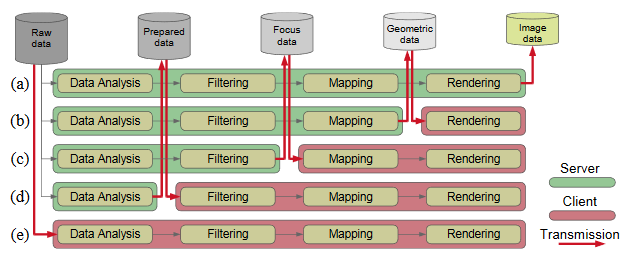
\includegraphics{./tex2pdf.19444/e0c5f6b5a33f6a7a2984bb5476a45bc971a5a5f2.png}
\caption{visualization pipeline in client-server scenarios}
\end{figure}

The raw data is stored on the server, sending the unprocessed data to
the client is a poorly performing approach. The provisioning of large
report files would take too long. Therefore the data need to be
pre-processed on the server. The client should be able to get the
pre-processed, but he can present only a subset of it in each view. One
user scenario is that the analyst takes just a short look into the
dataset. In this case he sees only one or a few views. Requesting the
complete set of data would result in long initial loading times for each
report. In an improved version the client request only the data the user
wants to see. Therefore the server subsets the data for specific
views.\\
Further work on the server side like mapping or rendering the data
({\textbf{???}}) would speed up the clients loading time enormously
({\textbf{???}}). But in the same scale it would increase the required
processing power on the server. For many clients this solution would not
be scalable. Because of that option \emph{c} in the figure will be
implemented.

The more generic reference model for data visualization by Ben
Shneiderman helps to further distinct the tasks between server and
client. The server will handle all data, while the client will present
the visual forms. The data transmission between the two components
should be implemented in a standardized way, which allow parameters for
the different views and files. The model distinct also the routing task
between client and server. The server makes the rooting between the
different files/data sources. He will route the client to the reporting
component for this file. The client on the other hand will handle the
routing between the different views inside the selected dataset.

\section{Backend technology
requirements}\label{backend-technology-requirements}

According the the architecture the backend has three main tasks: reading
data in different formats, analysis and pre-processing the data and the
provide the data in a standardized way. Additionally the backend need to
deliver the web pages to the clients.

The data provisioning should be implemented with stateless protocol. A
stateless protocol is simple to use and to implement. The simple
protocol makes the testing of the interface easier. A stateful
implementation would perform better a few clients, but with to many open
connections the application would crash. When using stateful protocol
the server would need to keep the large data tables in memory, and so
the application would scale badly. Another advantage is the loosely
coupling between client and server, this simplifies independent
development of front- and backend.({\textbf{???}}, \textbf{???})\\
The most common programming paradigm for stateless web request is REST.
The REST interface also improves the scalability of the application.
Since each query is context-free, each query needs the same amount of
resources. This makes it easier to scale the application and identify
bottlenecks in the application. When focusing on the frontend, the REST
API will not restrict the technology or language that can be used. This
enables this work to experiment with different frontend solutions
without changing the backend. It's also helpful for using different
types of frameworks based on the report type.\\
An emerging technology in this area is also GraphQL ({\textbf{???}}).
While GraphQL is great for performing highly specialized query's. It
adds unnecessary complexity to a simple API service ({\textbf{???}}).
Since the planned API provides only a subset of the report in a table
pattern, without any filter condition REST will be the better choice in
sense of complexity and maintainability.\\
Together with the web request the application has to handle normal HTTP
request to deliver the frontend application. For a reliable and fast
user interface these request should be handled by a fast and lightweight
web framework, with REST support.

Reading and analyzing the report data from different formats is the core
backend feature. The backend has to handle the diversity of the
different formats without deduction of performance or extreme
incensement in code complexity. Therefore the backend language should
provide fast I/O operations and libraries that can work on large data
sets. The libraries should be able to import, filter and provide
different kinds of as textual and tabular data. The backend should also
run scripts on the shell, to work with the binary blobs from profiling
tools.

\section{Dashboard technology
requirements}\label{dashboard-technology-requirements}

\subsection{Required frontend
components}\label{required-frontend-components}

The dashboard will be integrated in the existing application for
browsing the performance reports. The users doesn't need and want
another interface for viewing the reports, building another graphical or
web user interface would be counterproductive. This means the dashboard
development is web-based. A web-based application has also other
advantages for the use case like device diversity or bookmarking of
important views ({\textbf{???}}).

The web application is based HTML documents which will be styled by CSS
stylesheets. The dashboard has to react on user interactions, route
between views and needs to visualize structured data. To modify the
static HTML documents, most effort will go into the JavaScript(JS) code,
which is able to manipulate the existing Document Object Model (DOM) of
the HTML files.

To implement the frontend tasks, each task will be supported by at least
one frontend component. The components are simplifying the
implementation by providing different programming interfaces. The
frontend stack contains three components: a framework for building user
interfaces, a kit of style elements and visualization library

The UI framework is required to handle the user interaction to build and
route the different views. The styling components ensure a consistent
user experience and provide building bocks for the UI forms. The
visualization library is handle the frontend part of the visualization
pipeline. It will map the data into visual structures and render them.
The following three chapters analyze the requirements for each of these
components based on the use case study.

\subsection{Requirements for the UI
frameworks}\label{requirements-for-the-ui-frameworks}

The UI library will be chosen based on the following criteria's
separately per report module. The main reason for using such a library
should be to \textbf{improve programming speed}. Therefore a library
should only be chosen, to make the code more readable and add no
unnecessary extra complexity. The library should be lightweight,
flexible and \textbf{easy to integrate} in the current application
stack. As discussed before for the API interface the application and
therefore the frontend should be \textbf{scalable}. Effectively this
should also mean that the library has a \textbf{robust performance}. The
performance should also be testable without an extra application layer.
Finally, the library should be \textbf{stable} and good to trust. This
means it should be widely used or backed by a big company. Since this is
a cooperate work, all libraries have been available under a license
\textbf{free for commercial use}. The support for native development
will not be taken into account. (2)

\subsection{Requirements for styling
components}\label{requirements-for-styling-components}

On top of the the UI library styling components are necessary. These
improve the building speed and provide a consisted layout. The existing
layout application is based on Bootstrap version 3. Since the UI will be
extended extensively. The requirements for the new report modules are
the determining factor. The existing UI has only one view, changing it's
layout can be done without much effort. Independently on the chosen UI
Styling Component, it's must be used in the complete frontend to provide
an consisted User experience ({\textbf{???}}). Which design language the
User Interface is using is at this state of application not important.
The main User Experience (UX) requirements are reliability, speed and
flexibility to structure and interact on the interface ({\textbf{???}}).
Therefore styling frameworks with a \textbf{huge number of components}
are required. The dashboard have to react on user input, therefore the
framework needs a large part of form components. The components should
also be \textbf{reactive}, meaning the are designed for user
interaction. Instead of static components, they should be able to handle
their state by their own . This simplifies the development with the
components. On the other hand the framework should be lightweight, for a
good interaction speed. A \textbf{modular} UI kit can achieve this
balancing act. The framework should implement \textbf{modern features}
like grid breakpoints for Responsive Design and CSS Preprocessor support
for SASS or LESS. ({\textbf{???}})

\subsection{Requirements of visualization
libraries}\label{requirements-of-visualization-libraries}

While the UI library will handle all user interaction, the actual
visualization of the data has to be done by a charting library. For
these library counts the same as for the UI library, it has to be free
for commercial use. It also should be \textbf{independent of the chosen
framework} or on a huge amount of other libraries. UI-Frameworks have a
short lifecycle (3). This leaves the possibility to switch the
UI-Framework at a further time, without losing all effort brought into
the visualization. In general \textbf{compatibility} with different
UI-Frameworks and devices should be given. To ensure the future
compatibility the library should also be evaluated based on it's
continuous \textbf{enrichment and maintenance over time}. An active
project ensures also the \textbf{documentation} and so the development
effort to be expected. Since the data to be analyzed is huge, the
library should provide the best \textbf{performance} possible, taking a
more complicated implementation into account. It should also
\textbf{support the API format} in which the backend is providing the
data. The main goal of this work is to provide a highly customized
dashboard for the requirements of the Z performance analysts. Therefore
the library should provide a \textbf{wide range of visualization} and as
much \textbf{customization options} as possible to increases the options
in the visualization. ({\textbf{???}})

\chapter{Evaluation of the application
technologies}\label{evaluation-of-the-application-technologies}

\section{Data preparation and backend
technologies}\label{data-preparation-and-backend-technologies}

The existing backend is using a Flask({\textbf{???}}) environment on
Python for browsing the server's directories and dynamically render the
web pages with Jinga2({\textbf{???}}). This work aims to extend this
application. For reasons of efficiency keeping the existing code basis
would be helpful. Nevertheless if based on programming effort or
performance a switch of programming language or framework would be
necessary, this should be considered. This chapter will discuss benefits
of the different possible web backend's and highlight the best choice
for this application. Based on the choice of programming language the
possibilities for data preparation will be explained.

In extension to the current use scenario of the application will require
handling REST calls. The REST interface will be used by the clients to
access the rehashed report data ({\textbf{???}}).

To handle the web requests the backend requires web framework. According
to the Web Framework Benchmarks from TechEmpower ({\textbf{???}}), the
existing Python solution is not the fastest environment around.
Independently of the test type languages like Go, Scala, Java or C++ are
performing better than the Python frameworks. The majority of requests
against the web server will be REST requests for the analyzed data.
Looking at the TechEmpower benchmarks, the JSON serialization test runs
seem to match best our utilization scenario. When only looking at
request per seconds data, Java servlets are providing the best results
for JSON Serialization with about 560k queries. The best python library
is providing 87.5\% of the top performance. The best overall results for
plaintext queries are providing C and C++ with about 4 million queries.
Python reaches only 35.3\% of the top score.

The switch to Java or C/C++ would require a huge amount of time to set
up the new environment and rewrite the code. Since the application is
not meant to be a high-performance application, the extra amount of time
satisfies not the benefits. A good compromise between performance and a
simple to implement solution could also be Go(73.0\%) if performance
would get more important ({\textbf{???}}). Another try to improve
performance if it's getting necessary could be to switch to a more
performant web framework of python.

When taking a more specific look at python libraries in the TechEmpower
benchmark. It's quite clear that Flask is not providing the best
performance overall. The best-tested libraries for JSON and Plaintext
queries in mid-2017 seem to be falcon (432k /804k) and wheezy.web (377k
/956k). An older python specific benchmark test shows the same tendency
({\textbf{???}}). Both are not including a template engine for server
rendering. If this would be a necessary requirement bottle or weppy are
better alternatives. The TechEmpower benchmark is in no sense complete.
There are multiple fast and uprising web frameworks ({\textbf{???}})
like Sanic or Japronto. The latter promises about 1.2 million plaintext
queries per second ({\textbf{???}}), which would be even faster than the
fastest frameworks from the TechEmpower benchmarks. But since there are
not comparing in the same benchmark it's hard to compare them equally.
Ether way Flask seems to have only a quarter of the performance that is
possible in the Python environment. For further improvements in
performance, a switch to the falcon or wheezy.web framework should be
considered.

//DO why stay with flask

The current application is written in Python 3 and provides a web
application by using Flask. Flask is a slight web framework, which
provides a development server and the Jinja2 templating engine. The
Flask module enables the application to handle all web requests.

// How is Flask Working

//TODO
https://www.cabotsolutions.com/2017/11/a-detailed-study-of-wsgi-web-server-gateway-interface-of-python

Despite the fact that python may not be the fasted language
({\textbf{???}}) to solve this problem it has multiple other advantages.
Python is an interpreted language with a simple and readable syntax.
According to its author Guido van Rossum, one of the main concern when
developing the language was \enquote{\emph{to make Python code highly
readable}} ({\textbf{???}}). This goal has been fulfilled as shown in a
comparison based on expressiveness ({\textbf{???}}), where Python is
ranking significantly better than most other languages for this use
case. Even with the readable language design, the syntax keeps flexible,
when leveraging optional object-oriented or functional design patterns.
Altogether this minifies the development and debugging time. In terms of
efficiency, this is a huge cost saver and makes the application more
fault tolerant. On top of that python is great in combining different
technologies and languages and provides a comprehensive documenting
system with Sphinx ({\textbf{???}}). ({\textbf{???}}, \textbf{???})

Handling data structures in Python is simple compared to other
programming languages ({\textbf{???}}). This can be done also in other
languages which are providing even more libraries for different use
cases ({\textbf{???}}). But Python is providing the most efficient
libraries in terms of documentation and flexibility ({\textbf{???}}).
The main libraries that will be used in this application will be Pandas
and NumPy for reading and modifying the which is for most of the reports
table based. All other work like the visualization of the data will be
done on the front end.

To summarize this chapter, there are good alternatives for the backend
languages or frameworks. But until the performance of our application is
not getting the main concern. The current solution the most efficient
way to solve the given problems and develop the application. For the
project time frame of 7 weeks, this is equally important and therefore
the best tool of choice.

\section{Choose of frontend
technology}\label{choose-of-frontend-technology}

For further page loading improvements, the source code should be handled
by a module bundler. This will minify and optimize the code for
production by using transpilers.

//Explain more the frontend technology with article frontend for
dinosaurs

// Say something about huge continuous changes in technology
https://blog.logrocket.com/the-increasing-nature-of-frontend-complexity-b73c784c09ae

//babel and webpack here -\textgreater{} cite\\

\subsection{Dynamically updating the Document Object Model
(DOM)}\label{dynamically-updating-the-document-object-model-dom}

Based on the web statistics by W3Tech ({\textbf{???}}) jQuery is still
the most used JavaScript library to modify websites with JavaScript.
There are also multiple JavaScript Frameworks, which claim to be the
best (3). The main JavaScript-Framework competitors are React, Angular,
and Vue.js. Independent of the choice of framework, using such will slow
down the page loading as more powerful the framework gets. This means
plain or jQuery web pages are faster than a web pages build by a UI
framework ({\textbf{???}}). If a JS framework is required for the
building of an report interface, one of these three will be used instead
of jQuery or plain JS. Therefore these three will be evaluated in the
further comparison. Based on web page usage ({\textbf{???}}), the GitHub
stars ({\textbf{???}}) and the npm downloads({\textbf{???}}) React is
beating the other front-end frameworks. But as seen in ({\textbf{???}})
Vue.js is growing faster and may become the main competitor to React
({\textbf{???}}), whereas Angular has been beaten in this ranking.

The reason to use the jQuery library instead of plain JS with ECMA5
syntax is that it makes coding faster and easier to understand
({\textbf{???}}). Anyway adding the jQuery dependency to use only one
feature might not be reasonable, since there are always plain JS
solutions for a jQuery function ({\textbf{???}}). This is getting even
more enforced, since the latest specifications of JS EMCA6+ and now
upcoming EMCA2018 ({\textbf{???}}) have increase feature set of JS
({\textbf{???}}). The incompatibility of the newer specifications with
an older browser can be overcome by transpilers like babel.\\
In large projects, however, UI-Frameworks are handling better the
complex changes of the DOM. Where jQuery sites are requiring many
callbacks and event listener to handle asynchronous code execution,
frameworks are providing an interface to change the state of the page.
The huge amount of references in the plain JS based web pages makes it
harder to understand the code basis.

\subsubsection{Evaluated UI- Frameworks}\label{evaluated-ui--frameworks}

UI frameworks bring new features in the frontend without making the
source code unreadable. The web code written with a framework becomes
usually more modular and structured. This makes the application
components better testable and reusable. The framework makes it possible
to navigate between different subsites, without losing the data model or
loading a new HTML file. Each framework implements these features
slightly different. In the following they will be described shortly.

React describes itself as \enquote{a declarative, efficient, and
flexible JavaScript library for building user interfaces}
({\textbf{???}}). The first version was released in 2013, now 16.2.0
({\textbf{???}}) is the current version of the library maintained by
Facebook. The main characteristic of the library is the reactive
approach. This approach means if the state of a component changes React
is automatically rerendering the Virtual DOM ({\textbf{???}}), by using
its reconciliation algorithm ({\textbf{???}}). The Virtual DOM is a
virtual representation of the browser views in the memory. Applications
written in React are divided by their functionality into components.
This means JavaScript is generating the HTML by defining both business
logic and HTML markup ({\textbf{???}}). React used therefore a syntax
extension called JSX. Furthermore React is only a core library, it's
used in general together with React-Dom for the Virtual DOM in the
browser and several other extensions. ({\textbf{???}})

Whereas React is backed by Facebook, Google is behind the development of
Angular. The first version of Angular (AngularJS) was released in
October 2010. A complete has then been done into Angular2 (September
2016), on which all newer Angular Versions are based on. The current
version is 5.0.1. In contrast to its competitors, Angular relies on
Typescript. Typescript is an extension of JavaScript based on the
suggestions for EMCA6 developed by Microsoft ({\textbf{???}}). The main
features static typing and improvements for object orient concepts
({\textbf{???}}).\\
Angular has also a strict separation of technology and components. In
contrast to React Typescript is used to extend the HTML by creating HTML
\emph{templates} with Angularized markup. These templates are managed by
\emph{component} classes and the actual application logic is inside the
\emph{services}. Together they are boxed in \emph{modules}. Every
Angular App has a \emph{bootstrapping} the \emph{root module}, from
where on Angular takes over the navigation, presentation and user
interaction. This separation of different components follows strictly
the model-view-controller pattern. Additionally Angular is providing
most functions in its core dependencies and almost predefined workflow
for the development. ({\textbf{???}})

Vue.js is the youngest of the three frameworks, introducing it's the
first version in February 2014 and the current version 2 in 2016. It's
not developed by a big company, instead of by a small team of a dozen
developers led by Evan You. Even though large companies like Alibaba or
Baidu are using it. Vue.js has borrowed most of its concepts from its
successors like Angular, react or Ember.js. Like React Vue.js utilizes a
virtual DOM and provide reactive and composable view components. But
addition it integrates frequently used features like routing and global
state management in the core library. In contrast to Angular or React it
forces the user not to learn superset of JavaScript, like JSX or
Typescript. The top priority of Vue.js is to provide a lightweight and
easy to learn library for user views. ({\textbf{???}})

\subsubsection{Comparison of the UI
frameworks}\label{comparison-of-the-ui-frameworks}

All three libraries have their eligibility for different domains, the
evaluation will choose the best match based on the criteria defined in
the chapter before. All libraries are using the MIT license, so the k.o.
criteria of being used without any license cost are fulfilled.
({\textbf{???}}, Neuhaus.2017, (4))

In terms of programming speed, Vue.js is the best framework. According
to several articles, it has the fastest learning curve, together with a
very simple syntax that requires no extra technology like JSX or
Typescript. Not so easy to learn but also fast is React since it is only
a simple JS library to implement with great flexibility in the workflow.
Angular has a harder learning curve since it's very complex, but
Typescript (which is also available for React) improves the readability
of the code. In large projects, the scalability of the development time
is better with more developers.

All libraries are providing a solid documentation to learn the
framework.

In point of integration into the application environment, React and
Vue.js are equally straightforward. The reason behind this is, that both
are only JS libraries, which can easily be imported in normal JS files
without the need extra build dependencies like angular is requiring it.

The scalability can only be rated by way of deploying an application.
Angular brings its strengths in large Single Page Applications (SPA),
because it was build for them ({\textbf{???}}). Because of the strong
enforcement for modularity, large projects are better maintainable and
suitable for larger pools of developers. Angular is also easily testable
and therefore better scalable. React and Vue.js, on the other hand, can
more easily used for microservices, since they require only simple
imports of JS libraries. This enables better scaling for large
environments. React is even better for microservices since every
functional component of React is a single module. Because of the huge
amount of libraries React is also better for complex projects.

As shown in the js-framework-benchmark the frameworks cannot compete
with the fastest framework available. There compared performance is
almost one level. Vue.js is slightly faster, but the benchmark from
mid-2017 is also not using the newest versions aka React 16 and Angular
5. Especially in React 16 with React Fiber ({\textbf{???}}) has made
huge performance improvements under the surface. Important for the speed
of the initial page loading, can also be the library size. Since Vue.js
is the most lightweight it is in general faster, whereas Angular is the
slowest one.

React and Angular have the backing of two of the most powerful
companies, in financial aspects as well as in their skill in the area.
Vue.js, on the other hand, is founded via Patreon even tough it get used
by Baidu and Alibaba. Based on the npm downloads React is definitely the
most used framework of them three. React is also the most popular one
based on the stateofjs survey ({\textbf{???}}) and the GitHub stars
({\textbf{???}}). Even though the community of Vue.js is growing faster
at the moment.

React is the winner for this comparison based on the huge environment
supporting it and it's high popularity. The workflow of React is very
flexible so that it is easily integrated into the current application
environment. Vue.js stands out with a simple and lightweight framework,
which would make development, even more, easier than React. Even though
its only one of many uprising technologies. Vue.js may success React
({\textbf{???}}), but at this point of time React seems to be the more
safe choice of tool, since it's backed by a big company and the most
popular framework. It's also easy to start with and fulfills the
necessary requirements. So React is a good choice as the framework for
the more complex multipage sites.

https://medium.com/\textbf{???}

https://www.robinwieruch.de/reasons-why-i-moved-from-angular-to-react/

https://hackernoon.com/angular-vs-react-the-deal-breaker-7d76c04496bc

https://medium.freecodecamp.org/a-real-world-comparison-of-front-end-frameworks-with-benchmarks-e1cb62fd526c

https://hackernoon.com/5-best-javascript-frameworks-in-2017-7a63b3870282

https://medium.com/reverdev/why-we-moved-from-angular-2-to-vue-js-and-why-we-didnt-choose-react-ef807d9f4163

\subsection{Styling the User
Interface}\label{styling-the-user-interface}

The decision on the styling components has no huge effect on the
application. The styling components can be changed easily changed and
aesthetics are a matter of taste. The main requirements for the styling
components are that they can be used with different UI-Frameworks. The
support of different UI-Frameworks makes it easier to substitute the
underlying UI-Framework layer. The small reports may also only use
jQuery or even no library.

If IBM provides a suitable framework for the application this would be
the most consistent style component choice. At the moment internal
design framework for the internal w3 design is not publicly available.
IBM provides only the Carbon Framework ({\textbf{???}}) used by IBM
Cloud. This framework has not been chosen, because it provides not
enough form components for the user interaction. According to the GitHub
statistics Bootstrap, Semantic-UI, Foundation, Materialize and Material
UI are the five most popular UI-Frameworks. The frameworks have equal
features in most categories. All are licensed under MIT. Some are more
modular and performant that other, but the differences are to slight to
make a fundamental distinction. All have a responsive design and can be
used together with CSS preprocessors. The Foundation framework has only
a few form components and is unsuitable of complex user interaction.
There are also implementations of Material Design, Bootstrap and
Semantic UI for all common frameworks. This makes the choice for the
framework and aesthetic choice. I like the Material Design by Google the
most so I choose Material-UI for the React Framework and Materialize for
jQuery. ({\textbf{???}}, \textbf{???}, \textbf{???})

\subsection{Visualizing the data}\label{visualizing-the-data}

\subsubsection{Filtering visualization
libraries}\label{filtering-visualization-libraries}

Despite the user interactions on the dashboard, the data visualization
is the main focus of the dashboard. For efficiently creating a huge an
amount of plots for different views and datasets the use of a library
cannot be avoided. There many visualization libraries for JS. To get a
glue of the numbers, GitHub is listing about 850 JavaScript projects
(07.02.2018) under the term visualization ({\textbf{???}}). This chapter
can focus only on a subset of the available libraries. Since this work
relies on some mandatory requirements, libraries which not match the
following criteria will not be considered. The library must be open
source and \textbf{free for commercial use}. This disallows libraries
like Highcharts, FusionCharts, and ZingChart. Since the analyzed data is
confidential, the visualization has to be done \textbf{locally} without
leaving the Intranet. This prohibits API solutions like Google Charts
even if there are free or commercial use. To leave the possibility open
to switching the UI framework, the visualization library should not be
\textbf{depended on frameworks} ones like Ember Charts, Victory,
ReCharts or jqPlot. The reports are requiring a huge amount of different
charts which should ideally implement with only one library unless there
is a special use case which requires a special library. Therefore
specialized libraries like Timesheet.js, VivaGraph, Sigma.js, Leaflet or
heatmap.js are unsuitable. Only charting libraries are considered.

The focus report of this report is not a complete comparison of all JS
charting libraries. Only the most important libraries will be evaluated.
The distinction is done by GitHub star ranking and npm download
statistics. Only projects with over 1k stars and npm downloads per day
will be considered. This condition limits the list to D3.js, Chart.js,
C3, Raphael, NVD3, Chartist, ECharts, plotly.js, Vega, Vega-Lite and
Vis.js ({\textbf{???}}). In both rankings, D3.js and Chart.js are
completely outstanding. D3 is complete outstanding by even doubling both
numbers of Chart.js. In the further course of the chapter, the 10
different libraries will be shortly introduced with there main features
and then compared based on the criteria defined in chapter \textbf{XY}.

\subsubsection{Introduction of possible visualization
libraries}\label{introduction-of-possible-visualization-libraries}

The most popular library for data visualization is D3.js (5) also known
as D3 or Data Driven Documents. The library is based on Protovis and has
2 actively maintained versions v3 and v4. This evaluation will refer to
the newer (and better) version ({\textbf{???}}). One of the reasons for
the popularity is the flexibility of D3 ({\textbf{???}}). It is able to
manipulate the DOM and integrates the existing web technologies, like
Scalable Vector Graphics (SVG) and Canvas to create the visualizations.
The library can be used for any visualization project, because of it's
BSD 3-Clause, which allows commercial use as well. Using D3 for
different projects becomes even easier since D3 has a comprehensive API
documentation ({\textbf{???}}) and an own platform for example
visualizations with Bl.ocks ({\textbf{???}}). If some kind of
visualization not supported there is a high change a plugin to solve
this is already written, This list is proving an overview about the D3
plugins \cite{awesome-d3}. The visualization by D3 itself is fast and D3
can handle huge amounts of data compared to other libraries. The actual
speed of the rendering performance depends on the underlying technology.
Canvas is much faster the SVG graphics as shown in this performance
benchmark ({\textbf{???}}).

Many visualization libraries are using d3 and abstracting its complexity
and low-level interface to an easier to use interface. From the current
selection C3, NVD3, plotly.js, Vega and Vega-Lite are based on D3. Each
of the four libraries has different levels of abstraction
({\textbf{???}}).\\
NVD3.js has the highest level of abstraction of the four. The library is
developed by Novus Partners and distributed with the Apache 2.0 license.
The syntax is close to the original d3 library but only rudimental
documented and with a few possibilities. The library supports also only
the basic types of diagrams: bar, bullet, line and pie charts. Each of
the charts is provisioned with animations.\\
C3 indifference has a more extensive visualization API. The library is
developed since 2013 by Masayuki Tanaka under MIT license. The
visualization for C3 is done by a model definition in JSON. Compared to
NVD3 it has less visual effects. The API parameter, on the other hand,
are highly customizable and well documented. In contrast to NVD3, there
is also no more coding in d3 required. This makes it a lot easier to use
but, looses also the customization possibilities of d3.\\
Another D3 based library is called plotly.js. It's the JavaScript
implementation of the declarative Plotly API. The visualization
description exists for Python, Matlab, and R and is developed and
distributed by the Plotly Inc. under MIT license.The framework is built
on top of d3.js and stack.gl and provides over 20 different chart types.
The documentation side provides an extensive API description together
with many examples.

Like C3 or plotly.js, Vega ({\textbf{???}}) and Vega-Lite
({\textbf{???}}) are also declarative visualization languages based on a
JSON syntax. The languages are build by the Stanford Visualization
Group, now called the University of Washington Interactive Data Lab. The
same group that developed D3. Vega is not intended as a replacement for
D3 ({\textbf{???}}). Like D3 there are both licensed under the BSD-3
clause. D3 is meant to be a low-level visualization framework, whereas
Vega provides an abstract layer for representing and reasoning
visualizations. The idea behind the project is to \enquote{promote an
ecosystem of usable and interoperable tools, supporting use cases
ranging from exploratory data analysis to effective communication via
custom visualization design}. The abstraction layer has also various
improvements for Browser compatibility since there are translated in
runtime to D3 code based on the environment. Vega-Lite is based on Vega
and provides a higher level grammar to enable fast specification of
interactive data visualizations. Both libraries provide an enormous
amount of different charts and a very extensive documentation.

The main competitor of D3 according to usage stats is Chart.js. Like C3
or Vega, the charts are described with a JSON Model. The library
supports 8 highly customizable chart types, which cover almost all use
cases. Chart.js provides multiple examples for these charts and the API
is well documented. Chart.js is actively maintained by seven different
developers and published as Open Source with an MIT license. Chart.js
has good plotting performance using HTML5 Canvas. It also supports
responsive rerendering. Like D3 it also can be extended by plugins.

Raphael is a lightweight library for drawing vector graphics. It is
developed by Dmitry Baranovskiy under MIT license. In contrast to the
other libraries, it's the oldest release is a bit older than a year. The
library is easy to use for visualizations, but it is not scoped for
charts. This makes plotting charts harder to implement than in D3.
Especially for older devices or a great compatibility Raphael is a good
choice because of its unique support of the Vector Markup Language
(VML), SVG and Canvas objects.

Chartist is a lightweight charting library for customizable responsive
charts. Gion Kunz is the main developer of the library and licensed it
under MIT. Chartist can create three different kinds of plots bar, pie
and line charts. There are plotted into SVG and can be animated with the
Synchronized Multimedia Integration Language (SMIL). To implement the
charts, Chartist.js provides detailed examples and an API documentation.
Chartist is also extendable by plugins.

The vis.js visualization library ({\textbf{???}}) initially developed by
Almende B.V. and dual licensed under both Apache 2.0 and MIT. The
library designed to be easily usable and to handle large amounts of
dynamic data. The library consists of five main components: DataSet,
Graph2d, Graph3d, Network, Timeline. For the use case important is the
Graph2d component which plots data into bar or line charts. Pie charts
are not possible which makes the library unsuitable for the
visualizations purpose.

ECharts is a powerful charting library developed and maintained by
Baidu. ECharts provides a large number of possible visualizations in two
and three dimensional. The library is based on zrender, which uses
Canvas for the plotting, but ECharts is also available as a WebGL
version. It can also be integrated with several UI Frameworks or GIS
applications and has implementations in many other programming
languages. The JavaScript implementation is licensed under BSD 3-Clause.
The website provides many complex visualization implementations. The API
is documented in English and Chinese, even though the main language in
almost all user forums is Chinese.

\subsubsection{Decision on the best visualization
library}\label{decision-on-the-best-visualization-library}

The previous chapter has given a short overview about the most popular
JavaScript visualization libraries. This has only a small subset fitting
for the visualization requirements. The decision on the visualization
depends mainly on the balancing between simplicity and performance of
the implementation. If simplicity is more important Vega or even
Vega-Lite would be the considerable choice, elsewise if performance and
maximal customization is important D3 is the best choice. In the
following the decision on D3 will be explained on the establish
criteria.

The library should be compatible with a wide range of devices. This is
the case for all libraries, but in general the more high-level framework
s, like Vega are a bit more optimized in this criteria. The best
compatibility has Raphael. This is based on the support for old browsers
by VML.\\
On the other hand an chart implementation with Raphael would be very
hard, Vega-Lite is providing here the best compromise between
implantation speed and features.\\
Nevertheless the best feature set can only be reached with complex
low-level visualization framework. Besides the performance this is the
most important feature. The most feature rich libraries are D3 and
ECharts. But the problem with ECharts is that help for problem is only
available in Chinese language, where as D3 has an even larger English
community. Because of the huge user base, there are endless example
implementations for D3. D3 is also highly customizable and provides
almost any kind of chart ether natively or with a plugin. Additionally
it has also a great performance for a huge amount of data, which makes
D3 the perfect choice. ({\textbf{???}}, \textbf{???})

\chapter{Implementation of the
Dashboard}\label{implementation-of-the-dashboard}

This chapter will present an implementation overview based on the
architecture and technology decisions presented before. In the first
part the archtecture will be explained in detail. The second part will
present the key implementation in the back and frondend. The
implementation samples for the frondend will cover the REST API and the
data pre-proccessing. The samples for the frondend will cover the graph
plotting with D3, the visualisation of graphiz files and the page
routing with react.

\section{Dashboard architecture}\label{dashboard-architecture}

The application is designed with a two-tier client-server architecture
(S, 43ff, {\textbf{???}}). The advantage of this implementation \ldots{}

\begin{figure}
\centering
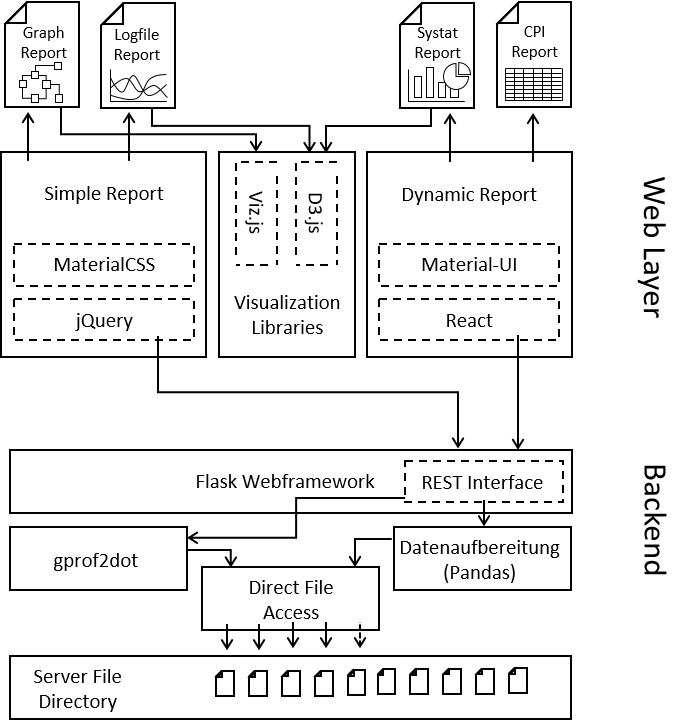
\includegraphics{./tex2pdf.19444/06fc6364987d51a2618f7bbaf6ec1533acca6cc2.png}
\caption{Dashboard Architecture Overview}
\end{figure}

\subsection{Application Frontend}\label{application-frontend}

https://hackernoon.com/a-map-to-modern-javascript-development-2017-16d9eb86309c

https://medium.freecodecamp.org/a-study-plan-to-cure-javascript-fatigue-8ad3a54f2eb1

At this point, the application is able to visualize four different kinds
of test files. The application visualizes the different parts of a
\emph{sysstat} report file in the sarcsv or sartxt format. It is also
able to interpret the outputs of different profiling tools like gprof or
perf by using the \emph{gprof2dot} script. The resulting dot files are
then shown at the web interface. Additionally, the tool is able to
visualize two other internally used file formats. It is interpreting log
files of the ML tests and so-called pureports, which are reports for
processing units.

Every kind of reports is an independent module of the application.
Therefore the separate reports don't have to be written using the same
technologies. For the presented visualizations this means that for the
complex or dynamic changing reports the React library is used for the
DOM manipulation. Whereas static reports are using the only jQuery for
DOM manipulations.

On the way of work, several CSS Frameworks for Material Design have been
tested. For static reports, MaterializeCSS has been chosen over Material
Design Lite. For React based reports Material-UI has is used. A detailed
argumentation for these decisions has been done in chapters \textbf{4}.

The main work effort in the frontend has been brought in the plots. A
report type can have multiple datasets, each of them is presented in an
own view. This view contains custom-designed plots visualised using the
D3.js library. D3.js is the library of choice because it provides the
highest scale of customization. More therefor in chapter \textbf{5} and
\textbf{6}.

Viz.js is handling the graphviz-files (dot) representation for the web.
The dot files can also be slightly manipulated by some custom JS
functions in the frontend.

The data for the D3 plots and the other interfaces are provided by a
REST interface. The REST interface is part of the Python project which
holds the complete backend logic.

\subsection{Application Backend}\label{application-backend}

The decision on python as backend has several reasons discussed in the
chapter \textbf{XY}. This decision has been taken because the previous
application was written in Python 3. 6 and the prototyping in python is
very fast for our use case. Python provides a lot efficient libraries
around data science and it has a simple and readable syntax.

The project has several dependencies. All web request is handled by
Flask, the REST interface as well as the rendering and the provision of
the web pages. The web provisioning part of the application has also
been extended about new routing rules for each report. Each report view
needs one or more REST requests. This is because only the data, that's
actually required should be sent to the client. Each REST Call is bind
to a function for the data preparation. Often the panda's library is
used for that since the majority of the data is tabular data. But there
are also a lot of other transformation, like separating the different
datasets in a report or finding matching lines in the ML-log files.

\section{Dashboard Implementation}\label{dashboard-implementation}

The second part will present the key implementation in the back and
frondend. The implementation samples for the frondend will cover the
REST API and the data pre-proccessing. The samples for the frondend will
cover the graph plotting with D3, the visualisation of graphiz files and
the page routing with react.

\subsection{Implementation of the backend
engine}\label{implementation-of-the-backend-engine}

\subsubsection{Data preprocessing in Python
3}\label{data-preprocessing-in-python-3}

\subsubsection{REST implementation with
Flask}\label{rest-implementation-with-flask}

\subsection{Implementation of visualisation and user
interface}\label{implementation-of-visualisation-and-user-interface}

\subsubsection{Page routing with React
v16}\label{page-routing-with-react-v16}

\subsubsection{Visualisation of Graphviz
files}\label{visualisation-of-graphviz-files}

\subsubsection{Data plotting with D3.js
v4}\label{data-plotting-with-d3.js-v4}

\chapter{Conclusions and future work}\label{conclusions-and-future-work}

::: What have been the requirements ::::::\\
Time\\
::: Architeture conclusion ::::::\\
Client Server Application

::: Technology conclusion ::::::\\
Best web framework = Flask, because is aready used -\textgreater{}
consider switching the web framework in python to wheezy or falcon\\
speak about Python vs.~Go\ldots{}???\\
Best UI-Framework -\textgreater{} react, vue may be a competitor\\
CSS Styling not important\\
Best Visualisation Framework -\textgreater{} D3

::: Implementation conclusion ::::::\\
- four reports, with difernet coverage and aspects -\textgreater{}
further work have to be done -\textgreater{} more reports, more plots
-\textgreater{} \ldots{}

::: Furthure Work ::::::

live stream data, while the report is running

single sign on ibm

berichte verbinden

::::::::::::::::::

\chapter*{Literature}\label{bibliography}
\addcontentsline{toc}{chapter}{Literature}

\hypertarget{refs}{}
\hypertarget{ref-Hottelet.2017}{}
1. HOTTELET, Ulrich. \emph{Der bilanzierte kunde: Der wert von daten für
die digitalökonomie} {[}online{]}. 2017. Berlin.
{[}Accessed~6~February~2018{]}. Available from:
\url{http://businessimpact.eu/der-bilanzierte-kunde/}Sie gelten als
Schmierstoff der Digitalökonomie und ihr Wert steigt und steigt:
(Kunden-)Daten sind das Öl des 21. Jahrhunderts.

\hypertarget{ref-Neuhaus.2017}{}
2. NEUHAUS, Jens. \emph{Angular vs. react vs. vue: A 2017 comparison --
unicorn.supplies} {[}online{]}. 2017. {[}Accessed~2AD--~6AD{]}.
Available from:
\url{https://medium.com/unicorn-supplies/angular-vs-react-vs-vue-a-2017-comparison-c5c52d620176}Deciding
on a JavaScript framework for your web application can be overwhelming.
Angular and React are very popular these days, and there\(\ldots\)

\hypertarget{ref-Allen.2018}{}
3. ALLEN, Ian. \emph{The brutal lifecycle of javascript frameworks}
{[}online{]}. 2018. {[}Accessed~6~February~2018{]}. Available from:
\url{https://stackoverflow.blog/2018/01/11/brutal-lifecycle-javascript-frameworks/}JavaScript
UI frameworks and libraries work in cycles. Every six months or so, a
new one pops up, claiming that it has revolutionized UI development.
Thousands of developers adopt it into their new projects, blog posts are
written, Stack Overflow questions are asked and answered, and then a
newer (and even more revolutionary) framework pops up to usurp the
throne.

\hypertarget{ref-DA14.2017}{}
4. DA-14 (ed.). \emph{5 best javascript frameworks in 2017}
{[}online{]}. 2017. {[}Accessed~2AD--~6AD{]}. Available from:
\url{https://da-14.com/blog/5-best-javascript-frameworks-2017}JavaScript
popularity continues its rising. In 2016 we've witnessed such great
changes, as AngularJS entire upgrade and introduction of Angular 2,
ultimate dominating of jQuery that is applied on 96.5\% of all JS sites,
evolution of ECMAScript, two updates of Node.js in April and October
accordingly, React finest hours, and even more. ~What to expect from
2017?

\hypertarget{ref-Bostock.2011}{}
5. BOSTOCK, Michael, OGIEVETSKY, Vadim and HEER, Jeffrey. D3:
Data-driven documents. \emph{IEEE Trans. Visualization \& Comp. Graphics
(Proc. InfoVis)} {[}online{]}. 2011. Available from:
\url{http://vis.stanford.edu/papers/d3}

\end{document}
